\documentclass{../../text-style}

\texttitle{Git, практика}

\begin{document}

\maketitle
\thispagestyle{empty}

На этой паре попрактикуемся в почти реальной командной разработке через GitHub --- попробуем разработать небольшую библиотеку командно, синхронизируясь через Git. Практика устроена так, чтобы конфликты были неизбежны (и это нормально, не надо пытаться их избежать административными мерами типа <<коммитим строго по очереди>> --- это и есть работа систем контроля версий). И, конечно, в реальной жизни всё происходит менее болезненно, чем, скорее всего, будет сейчас, потому что нам за одну пару надо прочувствовать боль где-то полугода командной разработки реальных проектов. Да, одному человеку сделать задачу будет быстрее, чем в команде, но мы не пишем код, а учимся.

Итак, задача очень простая: реализовать список на указателях/ссылках со следующими операциями:
\begin{itemize}
    \item Insert(int, object) --- добавить элемент по заданному индексу (индексация с нуля, Insert(0, ...) --- добавление в голову);
    \item RemoveAt(int) --- удалить элемент по заданному индексу;
    \item Get(int) --- получить элемент по заданному индексу (если ваш язык поддерживает переопределение квадратных скобок, используйте их);
    \item Set(int, object) --- установить элемент по заданному индексу;
    \item int Find(object) --- найти индекс по значению;
    \item int Count() --- узнать размер списка;
    \item Clear() --- очистить список.
\end{itemize}

Также, вторым приоритетом, реализовать для списка итератор так, как в вашем выбранном языке принято. И использовать генерики, если умеете.

Язык реализации может быть любой, лишь бы все члены команды умели на нём писать. На самом деле, я даже на конкретно этой задаче не настаиваю --- пойдёт всё, что можно поделить на содержательные подзадачи на 3-4 человека и успеть за пару в неторопливом темпе.

С организационной точки зрения сделать надо следующее.

\begin{enumerate}
    \item Поделиться на команды по 3-4 человека. Если это сложно, я могу случайно раскидать.
    \item Завести себе репозиторий на GitHub, один на команду. Тут уже вы внутри команды должны договориться, кто это сделает. Помните про README, лицензию и .gitignore. Чтобы выбрать правильный .gitignore, на этом этапе уже надо договориться о языке реализации.
    \item Расшарить репозиторий всем участникам. Это делается через интерфейс GitHub, в репозитории меню Settings -> Collaborators -> Add people. Для этого нужно, чтобы у каждого члена команды был аккаунт, и чтобы этот аккаунт знал хозяин репозитория. Если кто ещё не регистрировался на GitHub, самое время это сделать.
    \item Скинуть ссылку на репозиторий в чат курса, чтобы я мог по ходу дела наблюдать за вашими успехами.
    \item Завести внутрикомандный канал общения, какой вам угодно, хоть созвон в Discord.
    \item Кому-то одному завести и выложить проект и базовую инфраструктуру --- объявления методов, например, и общие типы (скорее всего, понадобится понятие <<узел списка>>).
    \item Поделить задачу на подзадачи и начать разработку по Git Flow. Можно не делать master с релизами и тэгами, можно master считать develop и вести всю разработку в нём. И у вас, видимо, не будет релизных и хотфиксных веток. Но обязательно разрабатывать каждую подзадачу в отдельной ветке и сливать изменения в master с помощью пуллреквестов, которые должны ревьюиться кем-то из сокомандников.
    \item Смотреть в чат команды --- я, возможно, буду комментировать происходящее. Возможно нет. В любом случае, вопросы стоит писать именно в общем чате.
    \item За 10 минут до конца собираемся и показываем, что получилось.
\end{enumerate}

Вот небольшое напоминание про Git Flow с прошлой пары:

\begin{center}
    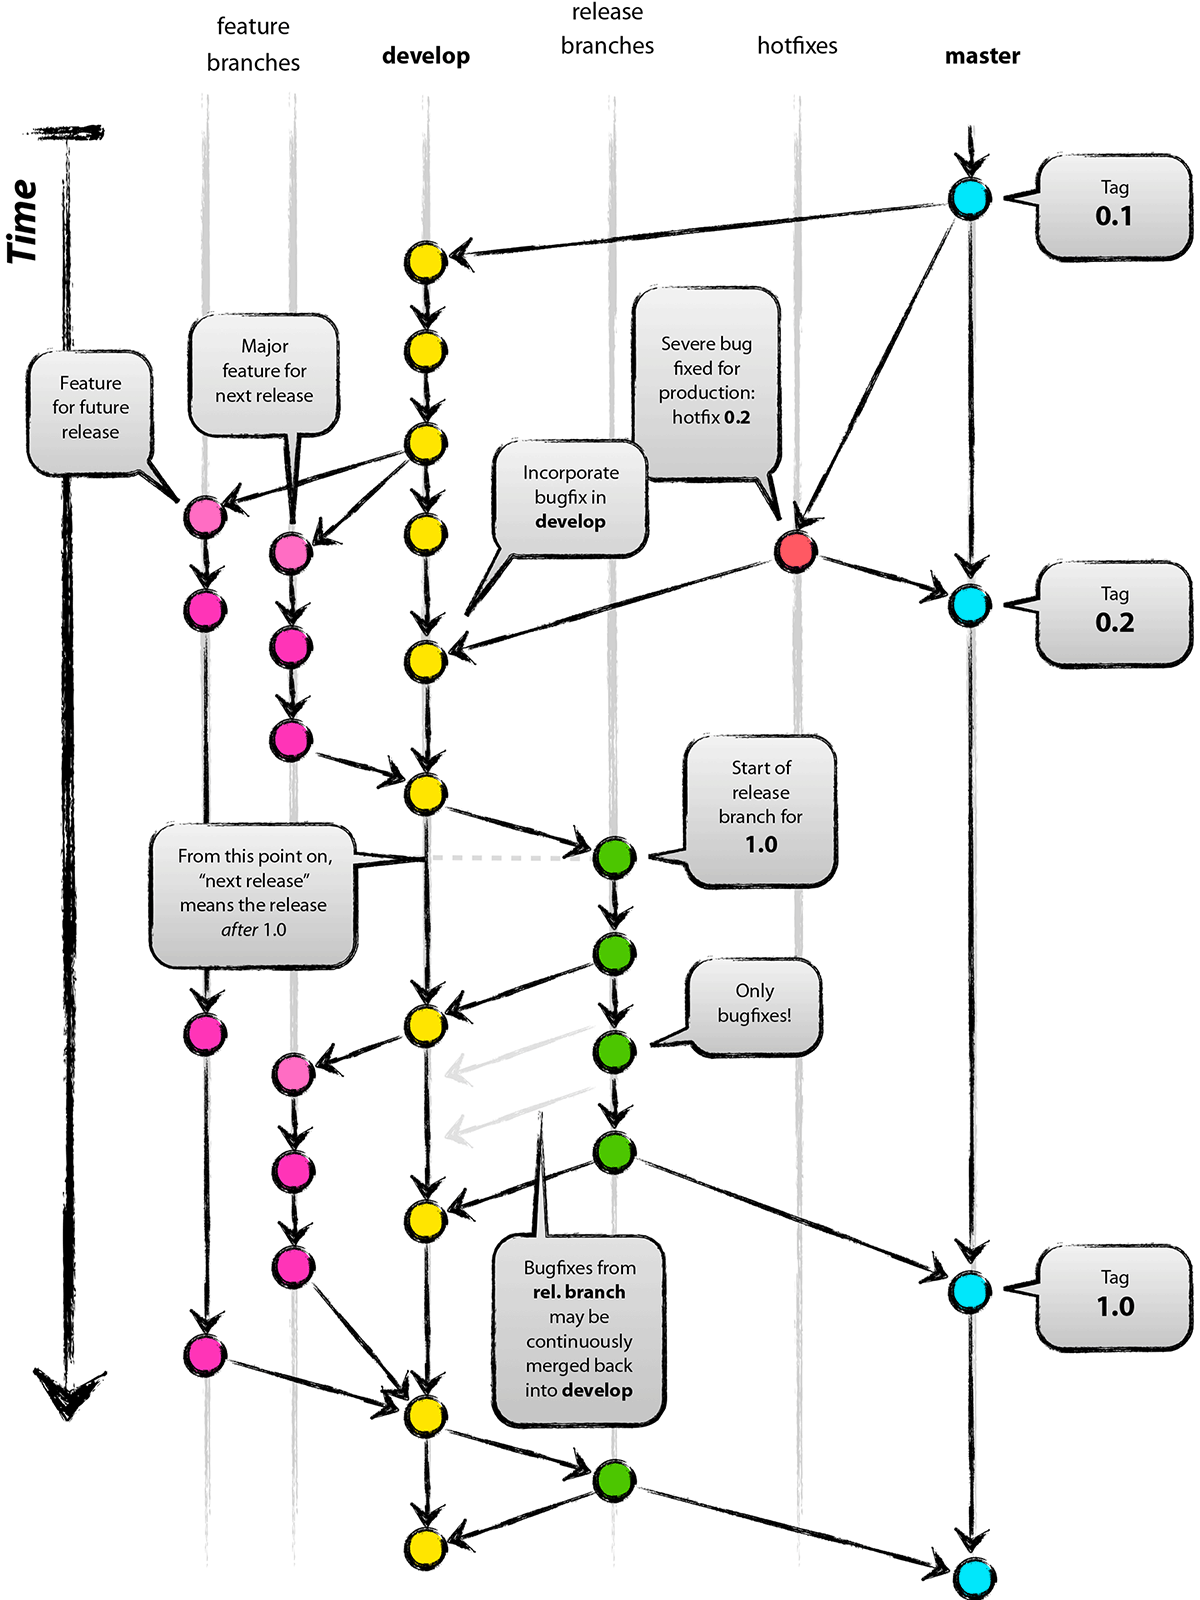
\includegraphics[width=0.4\textwidth]{gitFlow.png}
    \attribution{https://nvie.com/posts/a-successful-git-branching-model/}
\end{center}

\end{document}